%%%%%%% (stage)
\subsection{Concept of two-phase scheduling}\label{s:SchedHyperflow:PoC}

% \todo{Proof of Concept for DAG Scheduling in K8s}

%%% wrzuc zdjecia wykonan bez i z HEFT / PEFT i opisz przydzial na node'y (lub przykladowy schedule, lub oba)

% inquire
% drop wymiany kube-sched -> instead node-selectory + plugin

% Opisz ze korzystamy z HFlow + wstaw diagram z nodem, engine, plugin i scheduler + przejdz to K8s funkcji + wstaw diagram ze stanami dodanymi przy schedulingu

% Ze na inicjalizacji wyliczany jest plan, a potem w funkcji realizowane sa metody z interfejsu 

% pod z sched jest opcjonalny
%%

% To adopt 
The proposed concept for scheduling DAG-based workloads in Kubernetes consists of two phases, \emph{prioritization} and \emph{assignment}.
It is similar to the abstract idea of two-step scheduling proposed in Graphene \cite{b:Graphene}, which separates these responsibilities of a scheduler into independent steps -- ordering tasks for execution and then assigning resources to each one to run on.
In the prioritization phase, the tasks are being ordered to form an executable sequence.
After that, each of them waits for their turn until they can be executed.
The other phase is responsible for the process of assigning pods to the cluster nodes.
This part is handled entirely by the kube-scheduler.



%%% Przeedytuj zeby było wiadomo, dokładniej co się dzieje

% \begin{itemize}
%   \item{
% \emph{prioritization} -- in this phase, the tasks are being prioritized to form an executable sequence. After that, they are held in waiting before they can be executed 
% };
%   \item{
% \emph{assignment} -- a phase responsible for the process of assigning pods to the cluster nodes. It is handled by kube-scheduler.
% }
% \end{itemize}
% It is similar in an abstract idea to the two-step scheduling proposed in Graphene \cite{b:Graphene}, which separates these responsibilities of a scheduler into independent steps -- ordering tasks for execution and then assigning resources to each one to run on.


A conceptual representation of the necessary scheduling components for Hyperflow system in Kubernetes is shown in \cref{fig:solution:k8s-plugin-arch}.
The scheduler responsible for prioritization is included as a plugin to the Hyperflow engine.
The full implementation of the scheduler\footnotemark[1] and a template\footnotemark[2] to configure a new one are both shared for future reference.

\footnotetext[1]{Scheduler implementation: \url{https://github.com/Kmiet/hyperflow-dag-scheduler-plugin}, Access: 2021-07-20}
\footnotetext[2]{Scheduler template: \url{https://github.com/hyperflow-wms/hyperflow-simple-scheduler}, Access: 2021-07-20}

%%% Diagram node, z engine + pligun + sched
% Podpis diagraamu mowi ze sched jest opcjonalny i moze byc odpalony w podzie

%%%%
\begin{figure}[H]
\centering
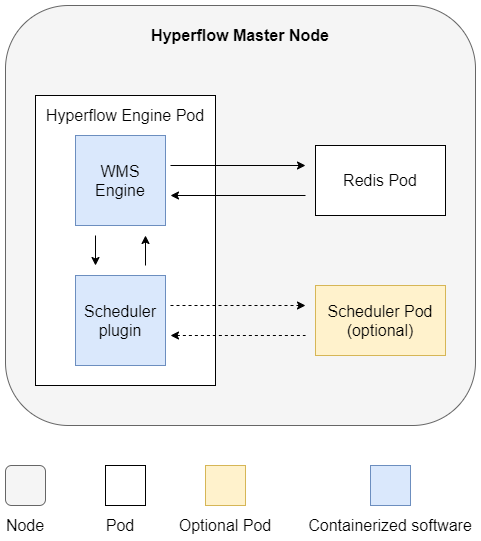
\includegraphics[width=0.5\linewidth]{figures/4-1-HflowPluginArch.png}
\caption[Concept of scheduling in Hyperflow]{Hyperflow master node in Kubernetes with scheduling components. The scheduler pod is an optional container deployed as a Kubernetes service. It is used to facilitate inclusion of scheduling algorithm with engine incompatible implementations.}

% \medskip
% \begin{minipage}{0.67\textwidth}
% {\footnotesize The scheduler pod is an optional container deployed as a Kubernetes service. It is used to facilitate inclusion of scheduling algorithm with engine incompatible implementations. \par}
% \end{minipage}

\label{fig:solution:k8s-plugin-arch}
\end{figure}
%%%%
\clearpage


% The plugin .. \todo{wrzuc zdanie o pluginie?}.
To be able to communicate scheduling decisions from the plugin to the kube-scheduler, all necessary information has to be sent in the workload deployment configuration.
% both scheduler decisions with each other \todo{(funkcje kubernetesa + pliki deployment -> node selector)}.
In \cref{fig:solution:k8s-states-single} all states of a modified single Hyperflow Kubernetes function are presented.
For static scheduling, a kube-scheduler is only responsible for pod-to-node assignment based on the provided node selectors.
Decisions on the availability of computing resources and their allocation are being handled by one of the scheduling algorithms.
Each resource identifier can be translated by the scheduler plugin to the matching cluster node selector.

\footnotetext[3]{HEFT Implementation: \url{https://github.com/mackncheesiest/heft}, Access: 2021-07-20}
\footnotetext[4]{PEFT Implementation: \url{https://github.com/mackncheesiest/peft}, Access: 2021-07-20}

%%% Tu diagram ze schematem działania schedulera -> interfejs WMS i sched -> K8s funkcja
% opis

%%%%
\begin{figure}[H]
\centering
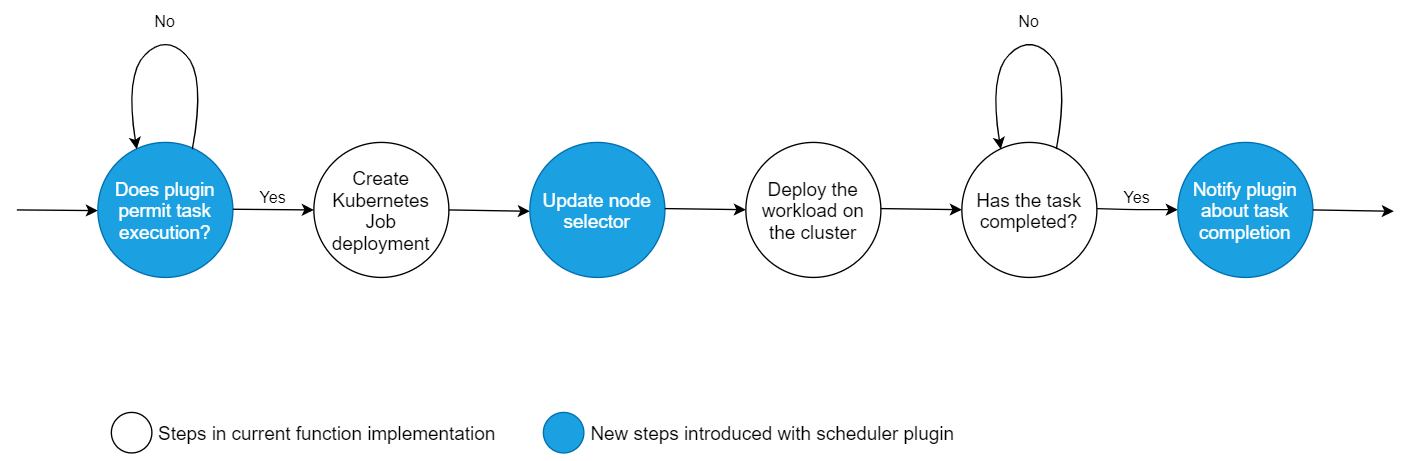
\includegraphics[width=1\linewidth]{figures/4-1-K8sFunction-2.png}
\caption[Adjusted Hyperflow function for Kubernetes workload scheduling]{States of an adjusted Hyperflow function for Kubernetes workload scheduling. The permissions from the scheduler plugin are a mechanism to ensure the correct order of execution for a single specific computing unit.}

% \medskip
% \begin{minipage}{0.65\textwidth}
% {\footnotesize The permissions from the scheduler plugin are a mechanism to ensure the correct order of execution for a single specific computing unit.\par}
% \end{minipage}

\label{fig:solution:k8s-states-single}
\end{figure}
%%%%


% The proposed concept for scheduling DAG-based workloads in Kubernetes is based on an idea similar to the two-step scheduling presented in Graphene \cite{b:Graphene}, which separates these responsibilities of a scheduler into independent steps -- ordering tasks for execution and then assigning resources to each one to run on.

% It is similar to the two-step scheduling proposed in Graphene \cite{b:Graphene}, which separates these responsibilities of a scheduler into independent steps -- ordering tasks for execution and then assigning resources to each one to run on.

For the experiment purposes, a pod with a static scheduler has been deployed and run as a Kubernetes service.
It supports a HEFT\footnotemark[3] and PEFT\footnotemark[4] algorithms for scheduling workflows.
To be able to plan the whole execution process, it is assumed that the necessary data of computation and communication costs for tasks are already provided at the workflow start.
With that input, a schedule is being computed using one of the selected algorithms.
The plugin then respects the order of task execution from the returned plan and grants permission for execution only for one task at a time on a single computing unit.

% -> Tu cos, pewnie wstep do omowienia planu lub nic


%%% Tu obrazek z planem wykonania prostego workflowu

% -> Tu cos lub nic


%%% Tu obrazek z wykonaniem prostego workflowu


The differences between a preplanned schedule and execution trace come from the lack of control over assignment to a specific computing unit (\cref{fig:solution:sched:plan-vs-trace}).
Therefore, on each subsequent execution, a container may have assigned a locally different processor, but of the same kind in terms of a physical resource.
For example, a pod may run on different cores of the same CPU.
This is guaranteed by the processor-to-node-selector translation, done within the scheduler plugin, which ensures a pod to be assigned and run on the same cluster.

%%%%
\begin{figure}[H]
\begin{subfigure}{1\textwidth}
\centering
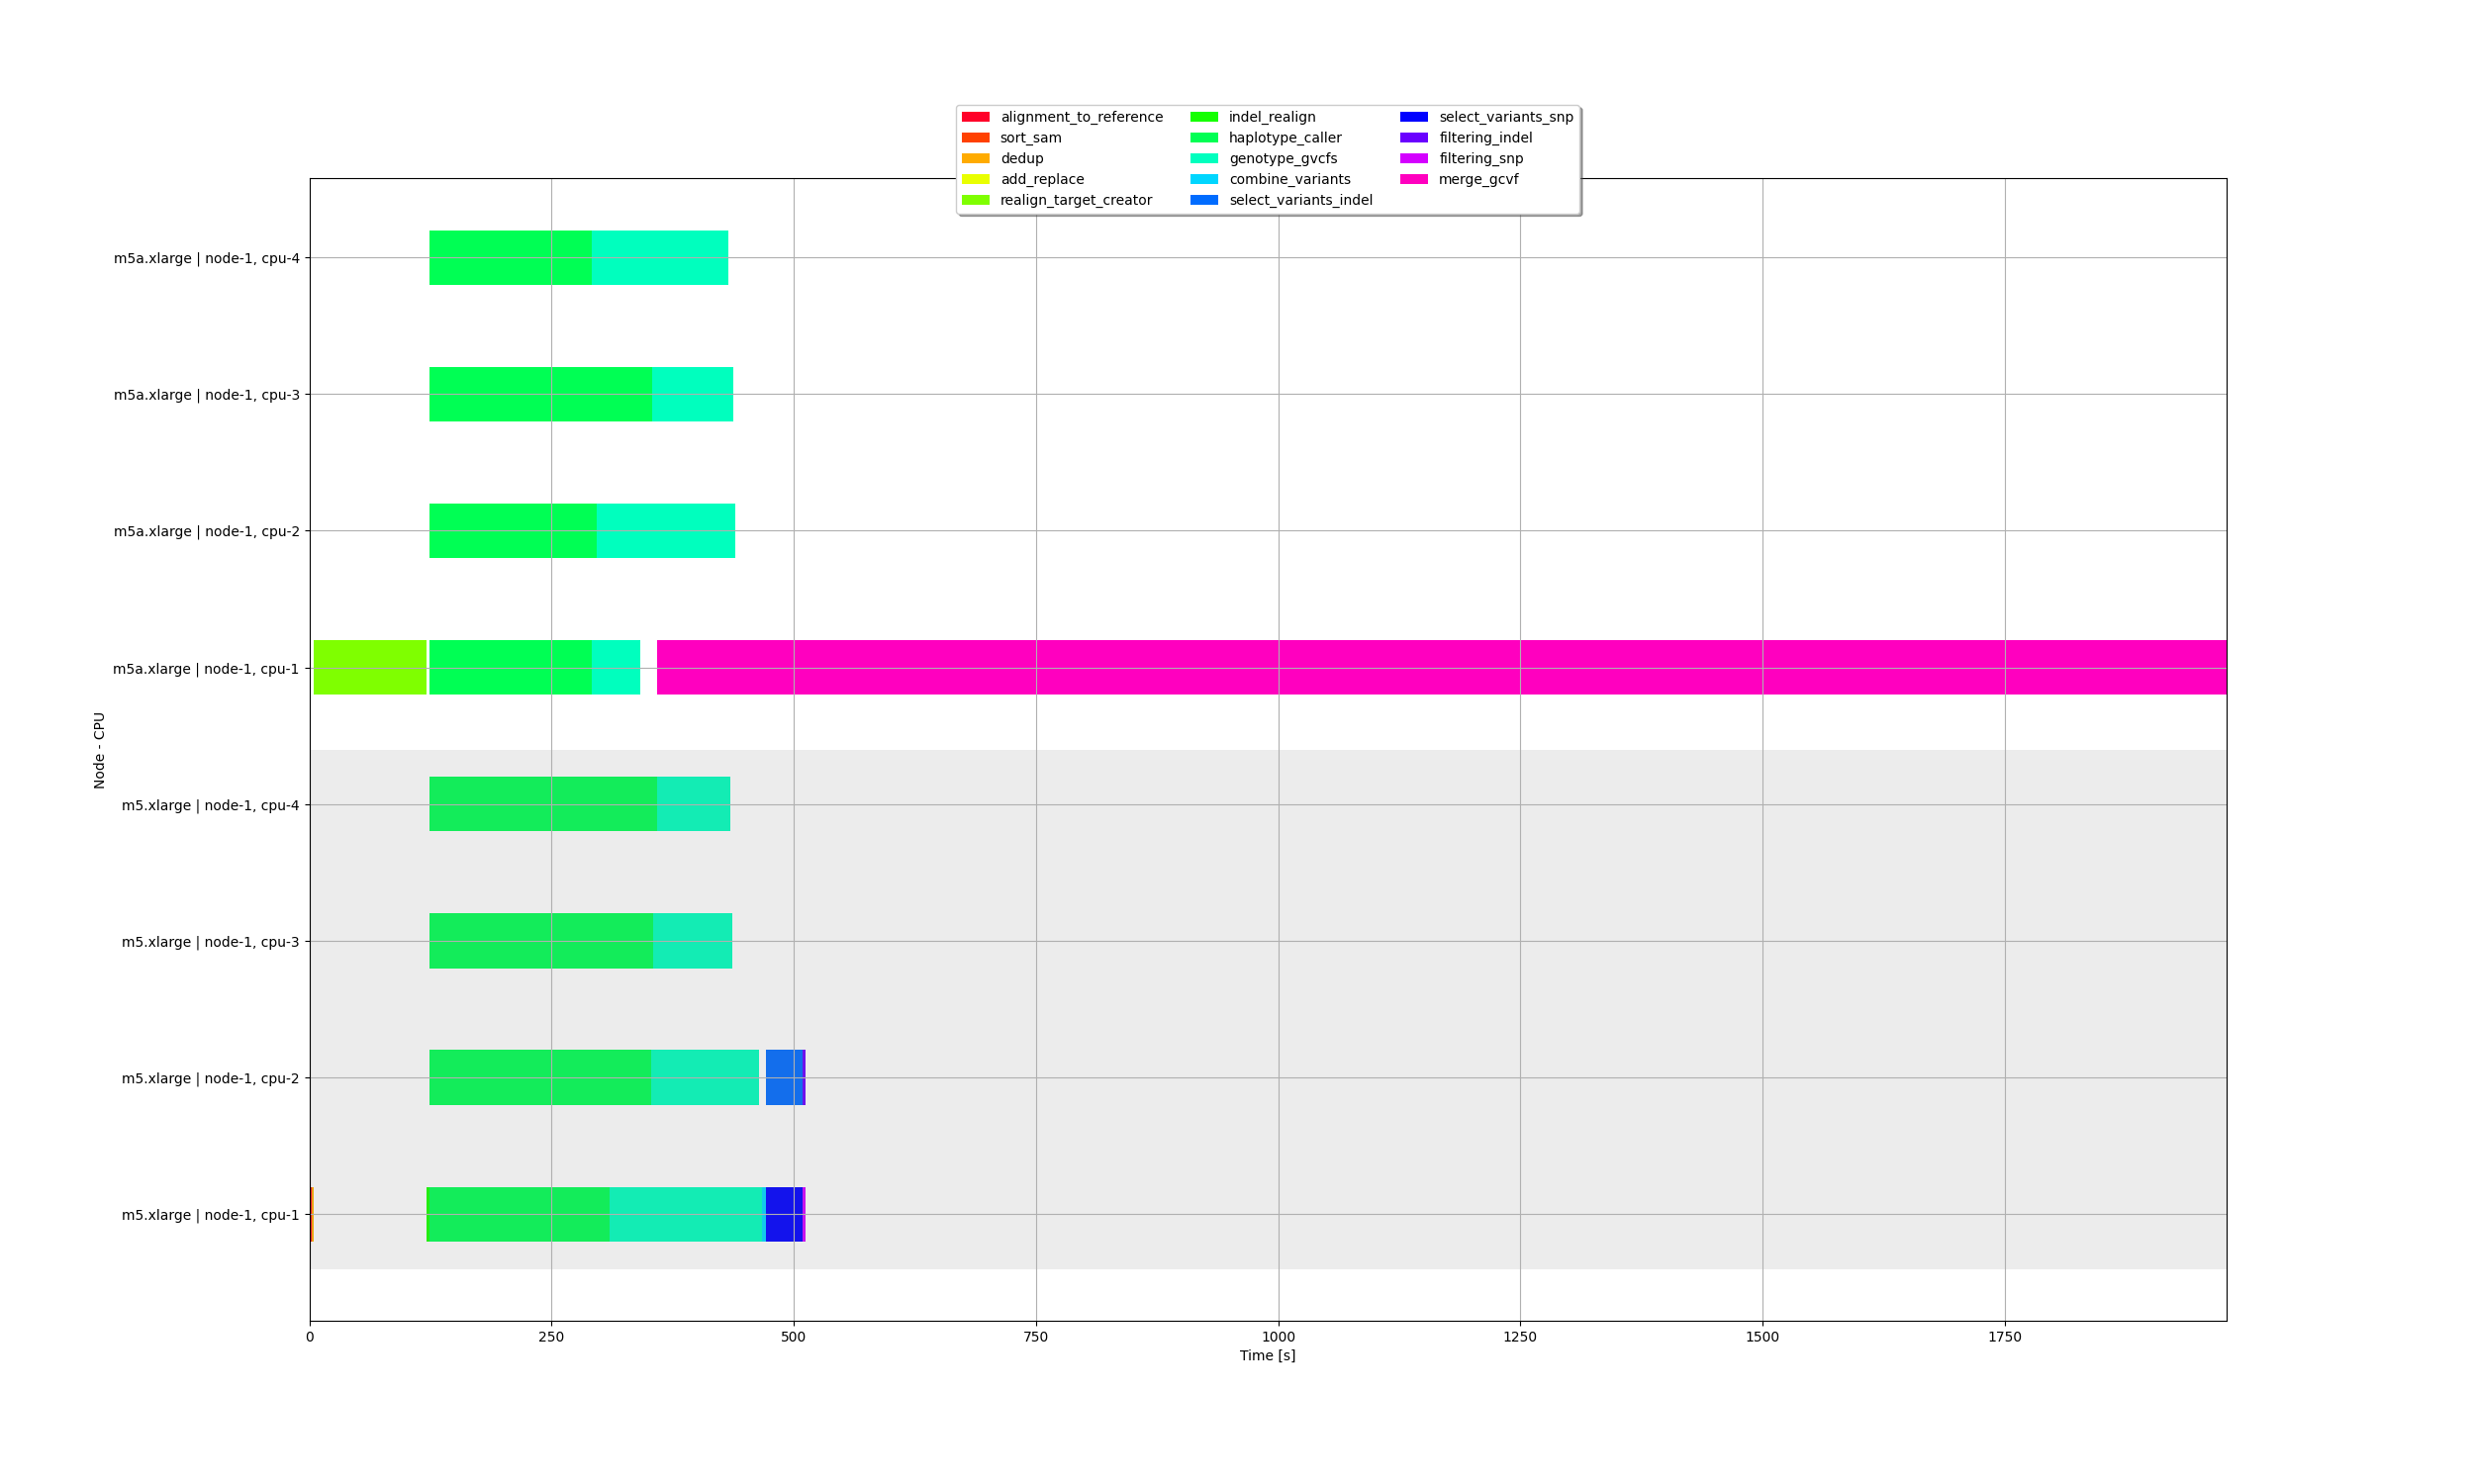
\includegraphics[width=1\linewidth]{figures/5-2-soykb_heft.png}
\caption[ScheduleOnly]{An examplary schedule computed with HEFT algorithm.} 
% \todo{Zmienić diagram na plan wykonania}}
\label{fig:solution:sched:plan}
\end{subfigure}
\begin{subfigure}{1\textwidth}
\centering
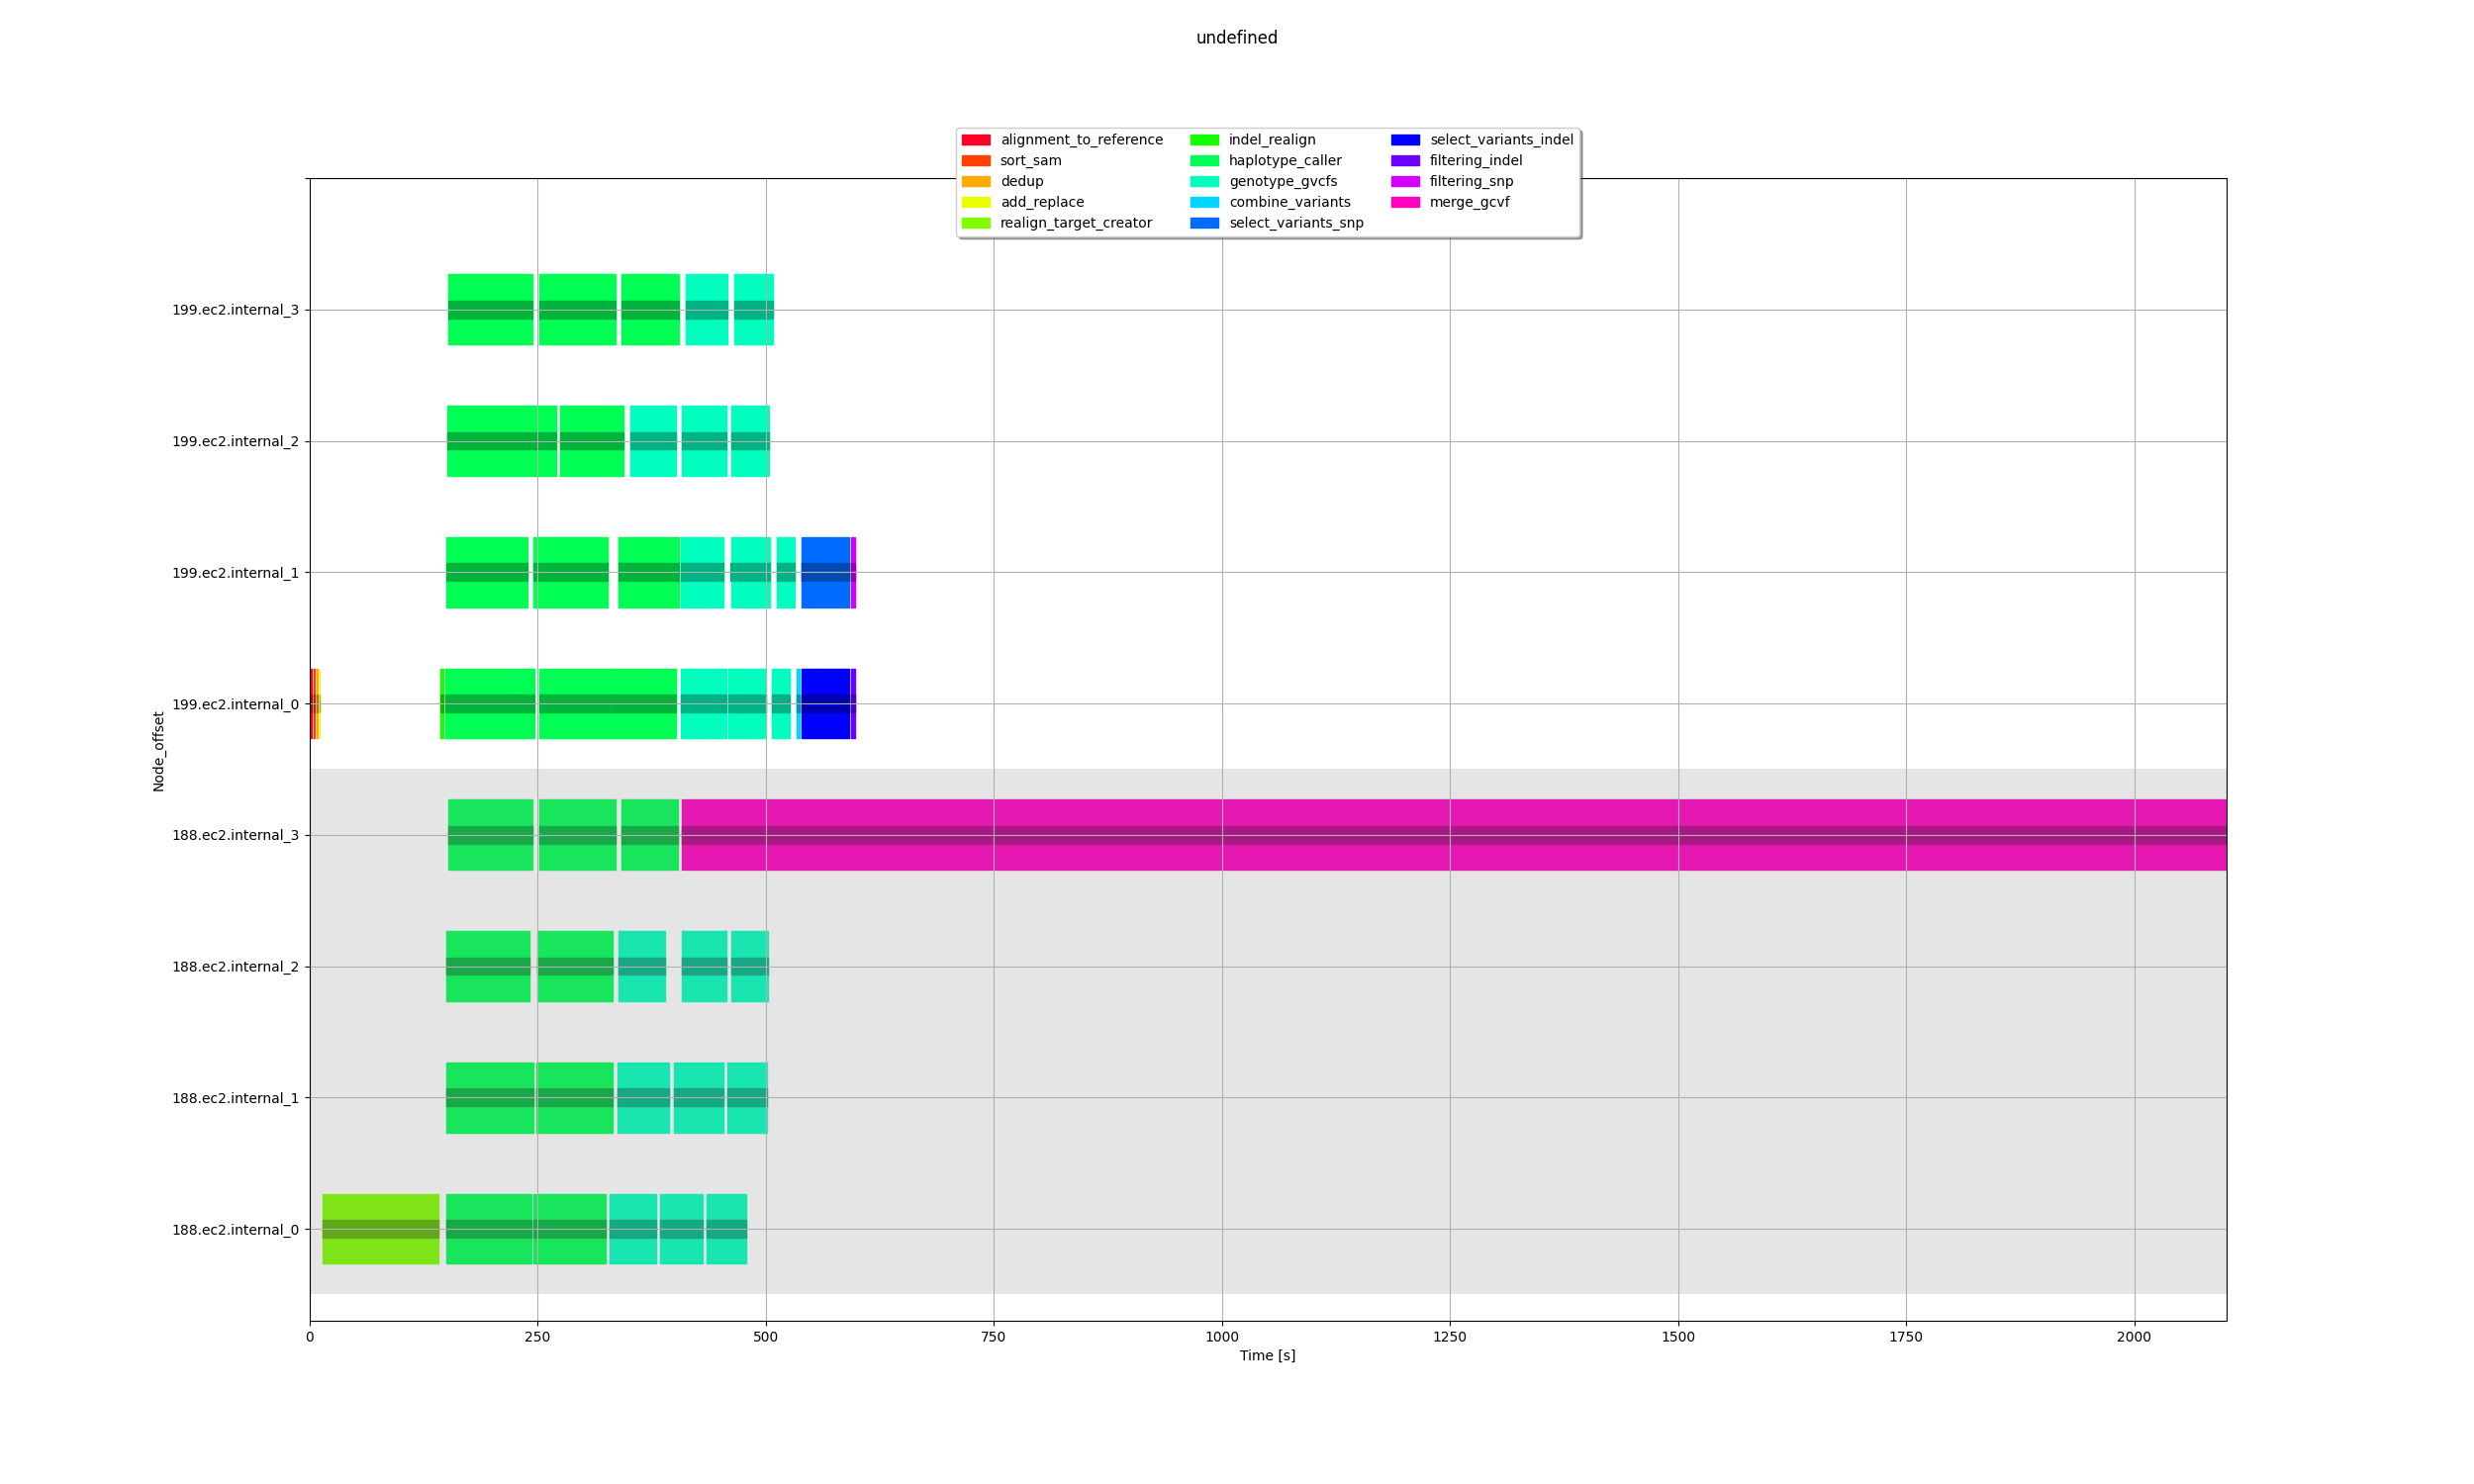
\includegraphics[width=1\linewidth]{figures/4-1-NoAgglo-HEFT.png}
\caption[ScheuleHEFT]{Execution trace for the computed plan from \cref{fig:solution:sched:plan}.}
\label{fig:solution:sched:heft}
\end{subfigure}
\centering

\caption[Differences between computed schedule and execution trace]{Differences in task to processor assignment between schedule and execution trace.}

% \medskip
% \begin{minipage}{0.75\textwidth}
% {\footnotesize Having no limitations on maximum buffer sizes allows creation of a single container with longer lifespan instead of multiple ones for a short periods of time. \par}
% \end{minipage}

\label{fig:solution:sched:plan-vs-trace}
\end{figure}
%%%%
